
\section{Séance 2}

\begin{exo}
Consid\'erez la grille $n \times n$, le graphe obtenu selon la Figure~\ref{fig:grille}, avec $n$ un naturel~$\geq 3$.
D\'emontrez que $n$ est pair si et seulement si le graphe est hamiltonien.
\end{exo}

\input{TP2/Figures/Grille.tikz}

Nous cherchons à prouver que tout graphe du style de la figure \ref{fig:grille} avec un n pair est un graphe hamiltonien. C'est à dire n pair $\Leftrightarrow$ graphe hamiltonien.

$\Rightarrow$ 

$\Leftarrow$ 

<C'est super long, et y'a des couleurs partout. TO DO plus tard.>

%-----------------------------------------------------------------

\begin{exo}
Prouvez que pour tout $n \geq 3$, le graphe complet $K_n$ poss\`ede exactement $\frac{1}{2}(n-1)!$ cycles hamiltoniens.
\end{exo}

\textbf{Cas de base} n=3, il s'agit d'un triangle. Ce graphe a $\frac{1}{2}(3-1)! = 1$ cycle hamiltonien.

\textbf{Récurrence} Supposons vrai pour $K_n$. Nous savons donc que $K_n$ possède $\frac{1}{2}(n-1)!$ cycles hamiltoniens. 

Pour $K_{n+1}$, nous construisons n cycles hamiltoniens supplémentaires en ajoutant le nouveau sommet entre 2 sommets quelconques de chaque cycle.

Donc, pour $K_{n+1}$ nous avons $\frac{1}{2}(n-1)!n = \frac{1}{2}n!$ cycles hamiltoniens.


%-----------------------------------------------------------------

\begin{exo}
Combien d'arbres couvrants poss\`edent les deux graphes de la Figure~\ref{fig:arbrecouvrant}?
\end{exo}

\begin{figure}[!h]
\centering
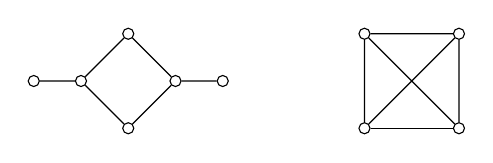
\begin{tikzpicture}[scale = 0.6]
\tikzstyle{every node}=[draw,circle,fill=black,minimum size=4pt,inner sep=0pt]
\node (a1) at (0,0) [shape= circle, draw, fill = white] {};
\node (a2) at (1,0) [shape= circle, draw, fill = white] {};
\node (a3) at (2,1) [shape= circle, draw, fill = white] {};
\node (a4) at (3,0) [shape= circle, draw, fill = white] {};
\node (a5) at (4,0) [shape= circle, draw, fill = white] {};
\node (a6) at (2,-1) [shape= circle, draw, fill = white] {};
\draw (a1) -- (a2) -- (a3) -- (a4) -- (a5);
\draw (a2) -- (a6) -- (a4);

\node (b1) at (7,-1) [shape= circle, draw, fill = white] {};
\node (b2) at (9,-1) [shape= circle, draw, fill = white] {};
%\node (b3) at (10,0) [shape= circle, draw, fill = white] {};
\node (b4) at (9,1) [shape= circle, draw, fill = white] {};
\node (b5) at (7,1) [shape= circle, draw, fill = white] {};
\draw (b1) -- (b2); -- (b3) -- 
\draw (b4) -- (b5) -- (b1) -- (b4) -- (b2) -- (b5);
\end{tikzpicture}
\caption{}
\label{fig:arbrecouvrant}
\end{figure}

\textbf{Graphe de gauche:} Il existe 4 arbres couvrants

\begin{figure}[!h]
\centering
\scalebox{.825}{\begin{tikzpicture}

\tikzstyle{every node}=[circle, draw, fill=white, inner sep=0pt, minimum size=5pt]

\node (v1) at (0,0) {};
\node (v2) at (1,0) {};
\node (v3) at (2,1) {};
\node (v4) at (3,0) {};
\node (v6) at (2,-1) {};
\node (v5) at (4,0) {};
\draw (v1) -- (v2) -- (v3) -- (v4) -- (v5);
\draw  (v6) edge (v4);
\node (v9) at (7,1) {};
\node (v12) at (7,-1) {};
\node (v10) at (8,0) {};
\node (v11) at (9,0) {};
\node (v8) at (6,0) {};
\node (v7) at (5,0) {};
\node (v18) at (12,1) {};
\node (v15) at (12,-1) {};
\node (v14) at (13,0) {};
\node (v13) at (14,0) {};
\node (v16) at (11,0) {};
\node (v17) at (10,0) {};
\node (v24) at (17,1) {};
\node (v21) at (17,-1) {};
\node (v22) at (18,0) {};
\node (v23) at (19,0) {};
\node (v20) at (16,0) {};
\node (v19) at (15,0) {};
\draw (v7) -- (v8) -- (v9) -- (v10) -- (v11);
\draw  (v12) edge (v8);
\draw (v13) -- (v14) -- (v15) -- (v16) -- (v17);
\draw  (v18) edge (v16);
\draw (v19) -- (v20) -- (v21) -- (v22) -- (v23);
\draw  (v22) edge (v24);
\end{tikzpicture}}
\end{figure}

\textbf{Graphe de droite:} Il existe 40 arbres couvrants. Trop nombreux pour que je les dessine tous.


%-----------------------------------------------------------------

\begin{exo}
Montrez que tous les alcools $C_nH_{2n+1}OH$ sont des mol\'ecules dont le graphe est un arbre, en sachant que les valences de $C, O$ et de $H$ sont respectivement $4, 2, 1$.
\end{exo}

<TO DO>

%-----------------------------------------------------------------

\begin{exo}
D\'emontrez que si un graphe hamiltonien $G = (V,E)$ est biparti selon la bipartition $V = A \cup B$, alors $|A|= |B|$. En d\'eduire que $K_{n,m}$, le graphe biparti complet, est hamiltonien si et seulement si $m=n \geq 2$.

\end{exo}

<TO DO>

%-----------------------------------------------------------------

\begin{exo}
Pour chaque graphe de la Figure~\ref{fig:graphes}, d\'eterminez si 
\begin{enumerate}
\item le graphe est hamiltonien,
\item le graphe est eul\'erien,
\item le graphe est biparti.
\end{enumerate}
\end{exo}

\begin{figure}[!h]
\centering
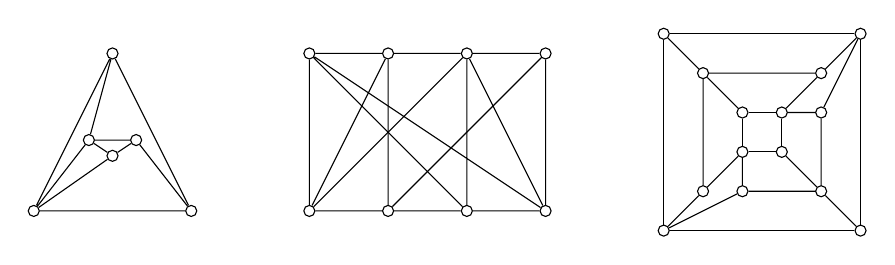
\begin{tikzpicture}[scale = 0.5]
\tikzstyle{every node}=[draw,circle,fill=black,minimum size=4pt,inner sep=0pt]
\node (a1) at (0,4) [shape= circle, draw, fill = white] {};
\node (a2) at (-2,0) [shape= circle, draw, fill = white] {};
\node (a3) at (2,0) [shape= circle, draw, fill = white] {};
\node (a4) at (0.6,1.8) [shape= circle, draw, fill = white] {};
\node (a5) at (-0.6,1.8) [shape= circle, draw, fill = white] {};
\node (a6) at (0,1.4) [shape= circle, draw, fill = white] {};
\draw (a1) -- (a2) -- (a3) -- (a1) -- (a5) -- (a2);
\draw (a2) -- (a6) -- (a4);
\draw (a3) -- (a4) -- (a5) -- (a6);

\node (a1) at (5,0) [shape= circle, draw, fill = white] {};
\node (a2) at (7,0) [shape= circle, draw, fill = white] {};
\node (a3) at (9,0) [shape= circle, draw, fill = white] {};
\node (a4) at (11,0) [shape= circle, draw, fill = white] {};
\node (b1) at (5,4) [shape= circle, draw, fill = white] {};
\node (b2) at (7,4) [shape= circle, draw, fill = white] {};
\node (b3) at (9,4) [shape= circle, draw, fill = white] {};
\node (b4) at (11,4) [shape= circle, draw, fill = white] {};
\draw (a1) -- (a2) -- (a3) -- (a4) -- (b4) -- (b3) -- (b2) -- (b1) -- (a1) -- (b2);
\draw (a1) -- (b3) -- (a4) -- (b1) -- (a3) -- (b3) ;
\draw (b2) -- (a2) -- (b4);


\node (a1) at (14,-0.5) [shape= circle, draw, fill = white] {};
\node (a2) at (14,4.5) [shape= circle, draw, fill = white] {};
\node (a3) at (19,4.5) [shape= circle, draw, fill = white] {};
\node (a4) at (19,-0.5) [shape= circle, draw, fill = white] {};

\node (b1) at (15,0.5) [shape= circle, draw, fill = white] {};
\node (b11) at (16,0.5) [shape= circle, draw, fill = white] {};
\node (b2) at (15,3.5) [shape= circle, draw, fill = white] {};
\node (b33) at (18,2.5) [shape= circle, draw, fill = white] {};
\node (b3) at (18,3.5) [shape= circle, draw, fill = white] {};
\node (b4) at (18,0.5) [shape= circle, draw, fill = white] {};

\node (c1) at (16,1.5) [shape= circle, draw, fill = white] {};
\node (c2) at (16,2.5) [shape= circle, draw, fill = white] {};
\node (c3) at (17,2.5) [shape= circle, draw, fill = white] {};
\node (c4) at (17,1.5) [shape= circle, draw, fill = white] {};

\draw (a1) -- (a2) -- (a3) -- (a4) -- (a1);
\draw (a1) -- (b1) -- (b2) -- (b3) -- (a3);
\draw (a1) -- (b11) -- (b4) -- (b33) -- (a3);
\draw (a2) -- (b2) -- (c2);
\draw (a4) -- (b4) -- (c4);
\draw (c1) -- (c2) -- (c3) -- (c4) -- (c1);
\draw (b1) -- (c1) -- (b11);
\draw (b33) -- (c3) -- (b3);
\end{tikzpicture}
\caption{}
\label{fig:graphes}
\end{figure}


\textbf{Graphe 1:}

\textbf{Graphe 2:}

\textbf{Graphe 3:}

%-----------------------------------------------------------------

